\documentclass[12 pt]{article}
%\usepackage[utf8]{inputenc}
\usepackage{amsmath}
\usepackage{amssymb}
\usepackage{geometry}
\usepackage{fancyhdr}
\usepackage{setspace}
%\usepackage{mathptmx}
\usepackage{newtxtext,newtxmath}
\usepackage{graphicx}
%\usepackage{lineno}
\usepackage[english]{babel}

\renewcommand\headrulewidth{0 pt}
\pagestyle{fancy}
\fancyhf{}
\rfoot{\thepage}
\lfoot{A temperature-driven model of phenological mismatch \\ Portalier, Candau \& Lutscher}
\lhead{
\includegraphics[height=1 cm, keepaspectratio]{JAE_Logo}}

\setstretch{2}

\geometry{tmargin=2.5 cm, bmargin=3 cm, lmargin=2.6 cm, rmargin=2.6 cm}

\begin{document}
\begin{Large}
\begin{center}
\textbf{Supplementary information}
\end{center}
\end{Large}
\begin{large}
\textbf{A temperature-driven model of phenological mismatch provides insights into the potential impacts of climate change on consumer-resource interactions} \\
\vspace{1 cm}
Portalier S.M.J.$^{1}$, Candau J.N.$^2$, Lutscher F.$^{1,3}$ \\
\end{large}
$^1$: Department of Mathematics and Statistics, University of Ottawa, Ottawa, ON, Canada \\
$^2$: Natural Resources Canada, Canadian Forest Service, Great Lakes Forestry Centre, Sault Ste. Marie, ON, Canada\\
$^3$: Department of Biology, University of Ottawa, Ottawa, ON, Canada \\
 
\vspace{0.5 cm}
\section{Theoretical developments}
In this supplementary material, we give the details for the mathematical derivation of the two sensitivity formulas for the end time of the seasonal resting period of a species. The general equation that connects the start time $t_0$, the rate curve $R(x)$ and the threshold $F$ to the end time $t^*$ of the resting period is

\stepcounter{equation}
\begin{equation}
    \int _{t_0} ^{t^*} R(x(t)) \mathrm{d}t = F. \tag*{Eq. S\theequation}
\end{equation}

\subsection*{General features}
We want to determine how $t^*$ changes when the temperature $x = x(t)$ changes by a small amount. More formally, we will derive a formula for the linear approximation

\stepcounter{equation}
\begin{equation}
    t^*(\epsilon) = t^*(0) + \epsilon \frac{d t^*}{d\epsilon} \tag*{Eq. S\theequation}
\end{equation}
where $\epsilon$ measures the magnitude of the small change, $t^*(0)$ is the end time when there is no change in the temperature time series from historical data, and the derivative is the sensitivity of the end time with respect to small changes. \par
We write the change in temperature as $x(t) + \epsilon z(t)$, where $z(t)$ is the pattern in which the temperature differs from the expectation and $\epsilon$ is small.  Since the end time now depends on $\epsilon$, we write $t^*=t^* (\epsilon)$.  The sensitivity of the end time with respect to $\epsilon$ is given by the derivative
\stepcounter{equation}
\begin{equation}
    \frac{\mathrm{d}t^*}{\mathrm{d}\epsilon} \; \text{for} \; \epsilon = 0. \tag*{Eq. S\theequation}
\end{equation}
This expression will depend on the pattern of temperature difference, $z(t)$. We will discuss two specific patterns below. \par

When we substitute these expressions into the defining equation for $t^*$ above, $\epsilon$ appears twice: once in the upper limit of integration and once in the integrand. To emphasize these two occurrences, we write the left-hand side of the equation as a function of two variables, namely
\stepcounter{equation}
\begin{equation} \label{Iequation}
    I(t^*(\epsilon),R(x+\epsilon x)) = \int _{t_0} ^{t^*(\epsilon)} R(x(t))+\epsilon z(t) \mathrm{d}t \tag*{Eq. S\theequation}
\end{equation}
When we differentiate the equation that defines the end time, $I(t^* ,R)=F$, with respect to $\epsilon$, we use the chain rule repeatedly and obtain
\stepcounter{equation}
\begin{equation} 
    \frac{\mathrm{d}}{\mathrm{d}\epsilon}I(t^*(\epsilon),R(x+\epsilon x)) = \frac{\partial I}{\partial t^*} \frac{\mathrm{d}t^*}{\mathrm{d}\epsilon}+\frac{\partial I}{\partial R} \frac{\mathrm{d} R}{\mathrm{d} x} \frac{\mathrm{d}x}{\mathrm{d}\epsilon} = 0 \tag*{Eq. S\theequation}
\end{equation}
The derivative of the integral in \ref{Iequation} with respect to the end time is simply the integrand evaluated at the end time. The derivative of the integral with respect to the integrand is the integral itself since this is linear. The derivative of the rate function with respect to $x$ is the usual derivative and the derivative of $x$ with respect to $\epsilon$ is $z$, by our definition above. Then we can solve the above equation for the quantity we are looking for and find
\stepcounter{equation}
\begin{equation} \label{dtdepsilon}
    \frac{\mathrm{d}t^*}{\mathrm{d}\epsilon}=\frac{- \int _{t_0} ^{t^*} R'(x(t)) z(t) \tag*{Eq. S\theequation} \mathrm{d}t}{R(x(t^*))}
\end{equation}
Hence, the end time has the linear approximation
\stepcounter{equation}
\begin{equation}
    t^*(\epsilon) \approx t^*(0)+\epsilon \frac{\mathrm{d}t^*}{\mathrm{d}\epsilon}=t^*(0)+\epsilon \frac{- \int _{t_0} ^{t^*} R'(x(t)) z(t) \mathrm{d}t}{R(x(t^*))} \tag*{Eq. S\theequation}
\end{equation}
As expected, the pattern by which the temperature deviates, $z(t)$, appears in this formula. We look at two interesting special cases for this pattern. \par

\subsection*{Specific patterns}
The first case is that the temperature change is constant throughout the period, independent of time. In that case, we can set $\epsilon z(t)=\Delta x$ to be the constant temperature difference. Then the function $z(t)$ drops out of the above integral and the end time is given by
\stepcounter{equation}
\begin{equation}\label{byconstant}
    t^*(\epsilon) \approx t^*(0) - \Delta x \frac{- \int _{t_0} ^{t^*} R'(x(t)) \mathrm{d}t}{R(x(t^*))} \tag*{Eq. S\theequation}
\end{equation}
Since $R'(x)>0$ and $R(x)>0$, the end time decreases if the temperature increases, i.e., the phenology advances. We knew this already from general consideration, but now we have an explicit expression for how much the advance is per degree increase. \par

The second case in which we can simplify the general formula is that there is a warm or cold spell of relatively short duration at a particular time during the resting phase. Then $\epsilon z(t)=\Delta x$ during the spell of duration $\Delta t$, starting at time $t_s$, and $z(t)=0$ otherwise. The integral in the numerator of \ref{dtdepsilon} can be approximated by
\stepcounter{equation}
\begin{equation}
    \epsilon \int _{t_0} ^{t^*} R'(x(t)) z(t) \mathrm{d}t = \Delta x \int _{t_s} ^{t_s + \Delta t}R'(x(t)) \mathrm{d}t \approx \Delta x \Delta t R'(x(t_s)) \tag*{Eq. S\theequation}
\end{equation}
Hence, the expression for the end time is approximately
\stepcounter{equation}
\begin{equation}\label{byspell}
    t^*(\epsilon) \approx t^*(0)-\Delta x \frac{\Delta t R'(x(t_s))}{R(x(t^*))} \tag*{Eq. S\theequation}
\end{equation}
This means that the end time is most sensitive to a warm or cold spell when the derivative of the rate function is the highest, all other things being equal. \par
The two formulas (\ref{byconstant} and \ref{byspell}) may seem different, but they express the same idea. One has to integrate $R'$ for all times where the two time series differ. When the two time series differ by a constant for all times, the one has to integrate over the entire time series. When the two time series differ only on an interval of length $\Delta t$, then one has to integrate over only that interval. If the interval is short, then the value of $R(x(t))$ does not change much and therefore the integral is approximated by the product of the length of the interval ($\Delta t$) and the value of the integrand ($R(x(t_s))$). 

\subsection*{Derivative of the rate function}
\stepcounter{equation}
\begin{equation}
    R(x)=\frac{1}{1+exp(b(x-c))}, \tag*{Eq. S\theequation}
\end{equation}
we can explicitly calculate the derivative as
\stepcounter{equation}
\begin{equation}
    R'(x)=\frac{-b exp(b(x-c))}{(1+exp(b(x-c)))^2}, \tag*{Eq. S\theequation}
\end{equation}
which is positive since $b$ is negative. To find the maximum of the derivative, we differentiate again and find
\stepcounter{equation}
\begin{equation}
    R''(x) = \frac{-b^2 exp(b(x-c))(1-exp(b(x-c)))}{(1+exp(b(x-c)))^3} \tag*{Eq. S\theequation}
\end{equation}
The maximum of $R’$ occurs where $R’’ = 0$, which happens when $x = c$ (see Fig. 2).

\section{Analysis of variance}
Here are the full results of the analysis of variance done on emergence date, budburst date and mismatch across latitude, for past/present temperatures, and for the three RCP scenarios. There are $6$ sites ranged from site 1 (southern site: $44.5^{\circ}$ N) to site 6 (northern site: $49.5^{\circ}$ N) (see Fig. 6 and main text for details). Analysis were performed with R.
\subsection{Past/present data}
\subsubsection*{Emergence date}

\begin{verbatim}
##              Df Sum Sq Mean Sq F value  Pr(>F)    
## Site          5   3374   674.8   17.89 3.2e-13 ***
## Residuals   120   4527    37.7                    
## 
## Signif. codes:  0 '***' 0.001 '**' 0.01 '*' 0.05 '.' 0.1 ' ' 1
\end{verbatim}

\begin{verbatim}
## 
##  Pairwise comparisons using t tests with pooled SD 
## 
##       Site1   Site2   Site3   Site4   Site5  
## Site2 0.20440   -       -       -       -      
## Site3 1.00000 0.64190   -       -       -      
## Site4 0.00574 1.00000 0.02647   -       -      
## Site5 2.0e-09 0.00021 2.0e-08 0.01493   -      
## Site6 1.5e-08 0.00102 1.4e-07 0.05283 1.00000
## 
## P value adjustment method: bonferroni
\end{verbatim}

\subsubsection*{Budburst date}

\begin{verbatim}
##              Df Sum Sq Mean Sq F value   Pr(>F)    
## Site          5   1332  266.43   21.72 1.94e-15 ***
## Residuals   120   1472   12.26                     
## 
## Signif. codes:  0 '***' 0.001 '**' 0.01 '*' 0.05 '.' 0.1 ' ' 1
\end{verbatim}

\begin{verbatim}
## 
##  Pairwise comparisons using t tests with pooled SD 
##  
##       Site1   Site2   Site3   Site4   Site5  
## Site2 0.21247   -       -       -       -      
## Site3 1.00000 1.00000   -       -       -      
## Site4 0.00062 1.00000 0.01185   -       -      
## Site5 6.5e-09 0.00050 3.5e-07 0.18502   -      
## Site6 3.1e-12 8.8e-07 2.2e-10 0.00155 1.00000
## 
## P value adjustment method: bonferroni
\end{verbatim}

\subsubsection*{Mismatch}

\begin{verbatim}
##              Df Sum Sq Mean Sq F value  Pr(>F)    
## Site          5  545.7  109.13   11.08 8.7e-09 ***
## Residuals   120 1182.1    9.85                    
## 
## Signif. codes:  0 '***' 0.001 '**' 0.01 '*' 0.05 '.' 0.1 ' ' 1
\end{verbatim}

\begin{verbatim}
## 
##  Pairwise comparisons using t tests with pooled SD 
## 
##       Site1   Site2  Site3   Site4  Site5 
## Site2 0.5382    -      -       -      -     
## Site3 1.0000  0.5175   -       -      -     
## Site4 0.2684  1.0000 0.2572    -      -     
## Site5 1.4e-07 0.0014 1.3e-07 0.0038   -     
## Site6 0.0042  1.0000 0.0039  1.0000 0.2517
## 
## P value adjustment method: bonferroni
\end{verbatim}

\subsection{RCP 2.6 data}
\subsubsection*{Emergence date}

\begin{verbatim}
##               Df Sum Sq Mean Sq F value Pr(>F)    
## Site     5 305237   61047    3334 <2e-16 ***
## Residuals   7194 131707      18                   
## 
## Signif. codes:  0 '***' 0.001 '**' 0.01 '*' 0.05 '.' 0.1 ' ' 1
\end{verbatim}

\begin{verbatim}
## 
##  Pairwise comparisons using t tests with pooled SD 
##  
##       Site1  Site2  Site3  Site4  Site5 
## Site2 <2e-16   -      -      -      -     
## Site3 <2e-16 <2e-16   -      -      -     
## Site4 <2e-16 <2e-16 <2e-16   -      -     
## Site5 <2e-16 <2e-16 <2e-16 <2e-16   -     
## Site6 <2e-16 <2e-16 <2e-16 <2e-16 <2e-16
## 
## P value adjustment method: bonferroni
\end{verbatim}

\subsubsection*{Budburst date}

\begin{verbatim}
##               Df Sum Sq Mean Sq F value Pr(>F)    
## Site     5  94260   18852    2896 <2e-16 ***
## Residuals   7194  46827       7                   
## 
## Signif. codes:  0 '***' 0.001 '**' 0.01 '*' 0.05 '.' 0.1 ' ' 1
\end{verbatim}

\begin{verbatim}
## 
##  Pairwise comparisons using t tests with pooled SD 
## 
##       Site1  Site2  Site3  Site4  Site5
## Site2 <2e-16   -      -      -      -    
## Site3 <2e-16 <2e-16   -      -      -    
## Site4 <2e-16 <2e-16 <2e-16   -      -    
## Site5 <2e-16 <2e-16 <2e-16 <2e-16   -    
## Site6 <2e-16 <2e-16 <2e-16 <2e-16 1    
## 
## P value adjustment method: bonferroni
\end{verbatim}

\subsubsection*{Mismatch}

\begin{verbatim}
##               Df Sum Sq Mean Sq F value Pr(>F)    
## Site     5  66174   13235    2316 <2e-16 ***
## Residuals   7194  41116       6                   
## 
## Signif. codes:  0 '***' 0.001 '**' 0.01 '*' 0.05 '.' 0.1 ' ' 1
\end{verbatim}

\begin{verbatim}
## 
##  Pairwise comparisons using t tests with pooled SD 
##  
##       Site1  Site2  Site3  Site4  Site5 
## Site2 <2e-16   -      -      -      -     
## Site3 <2e-16 <2e-16   -      -      -     
## Site4 <2e-16 <2e-16 <2e-16   -      -     
## Site5 <2e-16 <2e-16 <2e-16 <2e-16   -     
## Site6 <2e-16 <2e-16 <2e-16 <2e-16 <2e-16
## 
## P value adjustment method: bonferroni
\end{verbatim}

\subsection{RCP 4.5 data}
\subsubsection*{Emergence date}

\begin{verbatim}
##               Df Sum Sq Mean Sq F value Pr(>F)    
## Site     5 139304   27861    1045 <2e-16 ***
## Residuals   7194 191768      27                   
## 
## Signif. codes:  0 '***' 0.001 '**' 0.01 '*' 0.05 '.' 0.1 ' ' 1
\end{verbatim}

\begin{verbatim}
## 
##  Pairwise comparisons using t tests with pooled SD 
##  
##       Site1  Site2  Site3  Site4  Site5
## Site2 <2e-16   -      -      -      -    
## Site3 <2e-16 <2e-16   -      -      -    
## Site4 <2e-16 1.000  <2e-16   -      -    
## Site5 <2e-16 <2e-16 <2e-16 <2e-16   -    
## Site6 <2e-16 <2e-16 <2e-16 <2e-16 0.006
## 
## P value adjustment method: bonferroni
\end{verbatim}

\subsubsection*{Budburst date}

\begin{verbatim}
##               Df Sum Sq Mean Sq F value Pr(>F)    
## Site     5  51477   10295    1046 <2e-16 ***
## Residuals   7194  70813      10                   
## 
## Signif. codes:  0 '***' 0.001 '**' 0.01 '*' 0.05 '.' 0.1 ' ' 1
\end{verbatim}

\begin{verbatim}
## 
##  Pairwise comparisons using t tests with pooled SD 
## 
##       Site1  Site2  Site3  Site4  Site5 
## Site2 <2e-16   -      -      -      -     
## Site3 <2e-16 <2e-16   -      -      -     
## Site4 <2e-16 0.62   <2e-16   -      -     
## Site5 <2e-16 <2e-16 <2e-16 <2e-16   -     
## Site6 <2e-16 <2e-16 <2e-16 <2e-16 <2e-16
## 
## P value adjustment method: bonferroni
\end{verbatim}

\subsubsection*{Mismatch}

\begin{verbatim}
##               Df Sum Sq Mean Sq F value Pr(>F)    
## Site     5  23457    4691   651.4 <2e-16 ***
## Residuals   7194  51815       7                   
## 
## Signif. codes:  0 '***' 0.001 '**' 0.01 '*' 0.05 '.' 0.1 ' ' 1
\end{verbatim}

\begin{verbatim}
## 
##  Pairwise comparisons using t tests with pooled SD 
## 
##       Site1  Site2  Site3  Site4  Site5 
## Site2 <2e-16   -      -      -      -     
## Site3 <2e-16 <2e-16   -      -      -     
## Site4 <2e-16 0.22   <2e-16   -      -     
## Site5 <2e-16 <2e-16 <2e-16 <2e-16   -     
## Site6 <2e-16 <2e-16 <2e-16 <2e-16 <2e-16
## 
## P value adjustment method: bonferroni
\end{verbatim}

\subsection{RCP 8.5 data}
\subsubsection*{Emergence date}


\begin{verbatim}
##               Df Sum Sq Mean Sq F value Pr(>F)    
## Site     5 155376   31075   727.7 <2e-16 ***
## Residuals   7194 307197      43                   
## 
## Signif. codes:  0 '***' 0.001 '**' 0.01 '*' 0.05 '.' 0.1 ' ' 1
\end{verbatim}

\begin{verbatim}
## 
##  Pairwise comparisons using t tests with pooled SD 
## 
##       Site1  Site2  Site3  Site4  Site5
## Site2 <2e-16   -      -      -      -    
## Site3 <2e-16 <2e-16   -      -      -    
## Site4 <2e-16 0.202  <2e-16   -      -    
## Site5 <2e-16 <2e-16 <2e-16 <2e-16   -    
## Site6 <2e-16 <2e-16 <2e-16 <2e-16 0.014
## 
## P value adjustment method: bonferroni
\end{verbatim}

\subsubsection*{Budburst date}

\begin{verbatim}
##               Df Sum Sq Mean Sq F value Pr(>F)    
## Site     5  58046   11609   690.5 <2e-16 ***
## Residuals   7194 120951      17                   
## 
## Signif. codes:  0 '***' 0.001 '**' 0.01 '*' 0.05 '.' 0.1 ' ' 1
\end{verbatim}

\begin{verbatim}
## 
##  Pairwise comparisons using t tests with pooled SD 
##  
##       Site1   Site2   Site3   Site4   Site5  
## Site2 < 2e-16   -       -       -       -      
## Site3 8.2e-16 < 2e-16   -       -       -      
## Site4 < 2e-16 0.0097  < 2e-16   -       -      
## Site5 < 2e-16 < 2e-16 < 2e-16 < 2e-16   -      
## Site6 < 2e-16 < 2e-16 < 2e-16 < 2e-16 < 2e-16
## 
## P value adjustment method: bonferroni
\end{verbatim}

\subsubsection*{Mismatch}

\begin{verbatim}
##               Df Sum Sq Mean Sq F value Pr(>F)    
## Site     5  25363    5073   572.3 <2e-16 ***
## Residuals   7194  63763       9                   
## 
## Signif. codes:  0 '***' 0.001 '**' 0.01 '*' 0.05 '.' 0.1 ' ' 1
\end{verbatim}

\begin{verbatim}
## 
##  Pairwise comparisons using t tests with pooled SD 
## 
##       Site1   Site2   Site3   Site4   Site5  
## Site2 < 2e-16   -       -       -       -      
## Site3 < 2e-16 < 2e-16   -       -       -      
## Site4 < 2e-16 1       < 2e-16   -       -      
## Site5 < 2e-16 < 2e-16 < 2e-16 < 2e-16   -      
## Site6 < 2e-16 < 2e-16 < 2e-16 < 2e-16 1.1e-11
## 
## P value adjustment method: bonferroni
\end{verbatim}

\clearpage
\begin{figure}[ht]
\begin{center}
\renewcommand{\thefigure}{S\arabic{figure}}
\setcounter{figure}{0}
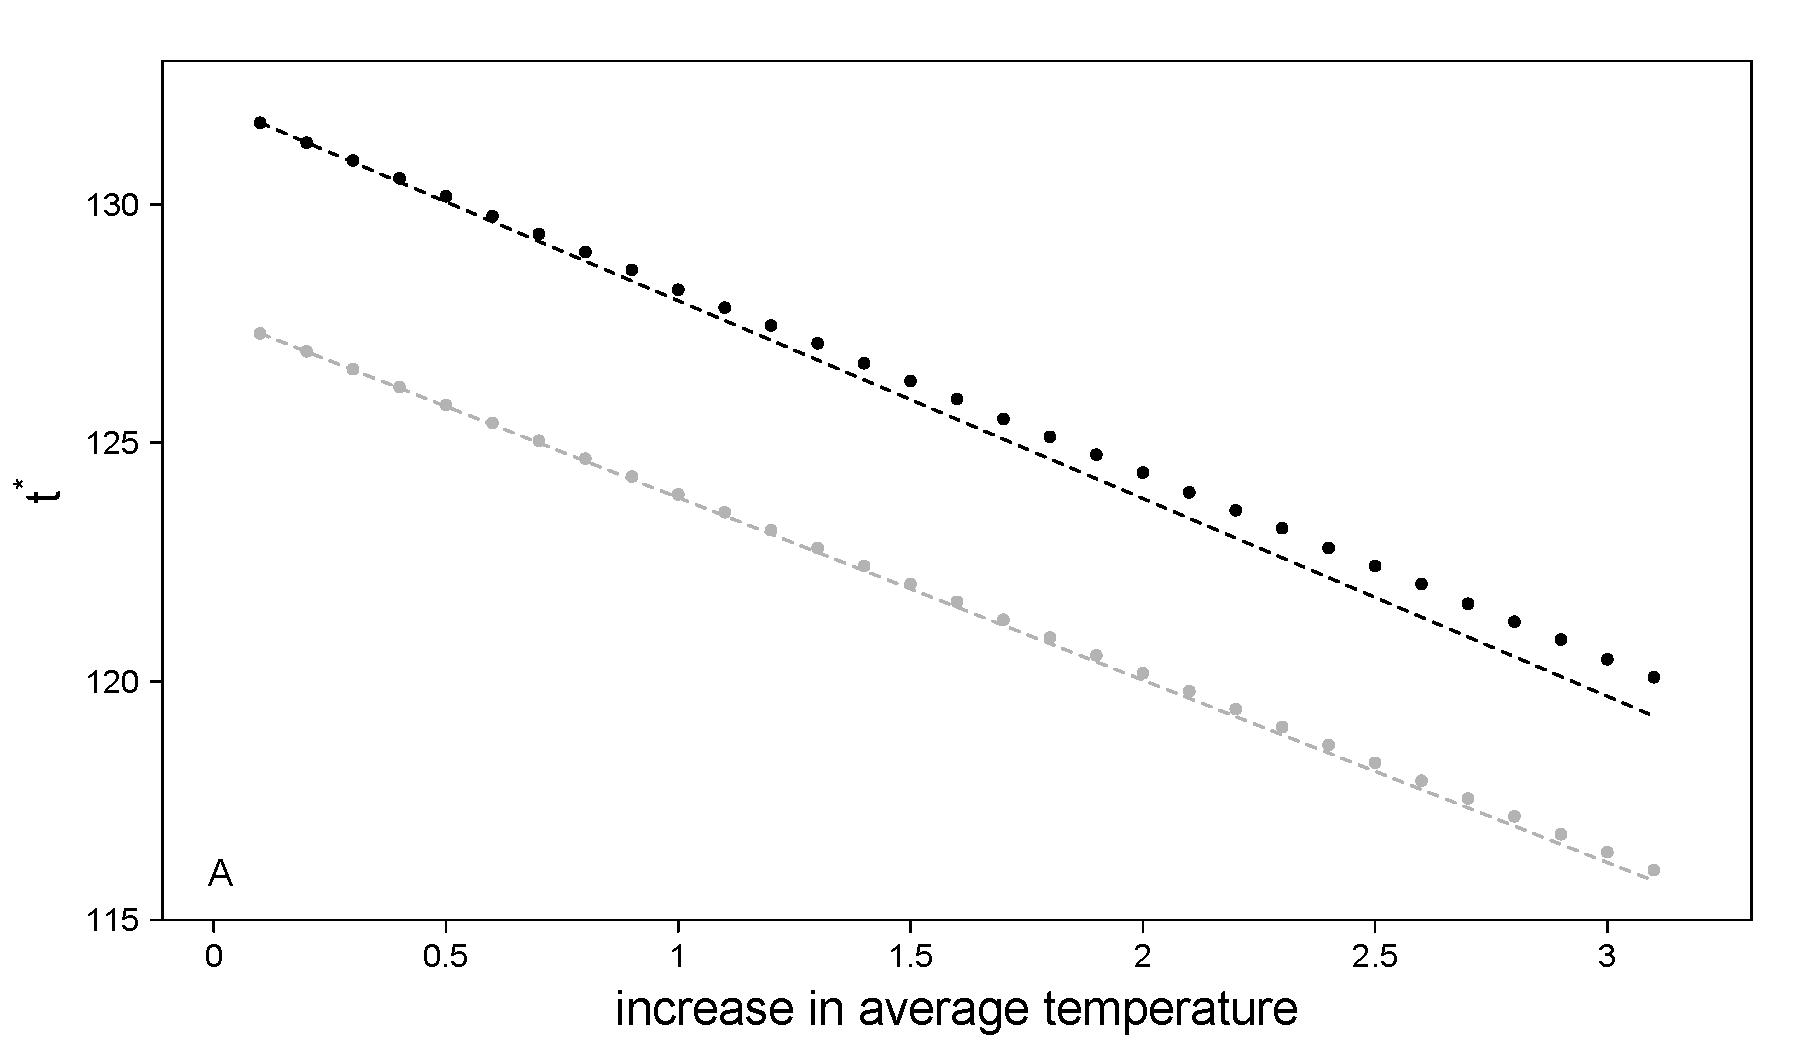
\includegraphics[width = 16 cm, keepaspectratio]{FigureS1}
\caption{\doublespacing Effects of a constant temperature difference on species phenology. Black is the consumer (SBW), and grey is the resource (balsam fir). A constant temperature difference advances species phenology. Dotted is the predicted value (Eq. 3 used with the $R$ functions of SBW and balsam fir), dashed is the linear approximation from the model with simple time series.}
\end{center}
\end{figure}
\end{document}